% Some commands used in this file
\newcommand{\package}{\emph}
\chapter{Introduction}
\label{ch:intro}
\chapterprecishere{"I had no idea this was going to be an accurate prediction, but amazingly enough instead of 10 [years] doubling, we got nine over the 10 years, but still followed pretty well along the curve."}{\hfill -- Gordon E. Moore\footnote{Computer History Museum Presents The 40th Anniversary of Moore's Law with Gordon Moore and Carver Mead (\url{http://goo.gl/4WT2ux})}

In 1965 Godon E. Moore, one of the founders of Intel, published his observation that the number of transistors on a chip of same size doubles approximately every 24 months and predicted similar exponential growth for the future \cite{moore_cramming_1965}. The so-called ``Moore's Law'' is illustrated in figure \ref{fig:moore_data}. A higher level of integration usually goes hand in hand with increasing performance. The availability of greater computational capabilities does not only accelerate existing solutions, but may enable applications from a variety of research fields that were previously impossible to realize or had been completely out of scope a few years ago. 

One of these fields is biochemistry. Over the years, computational methods have become a valuable and integrative tool that is by no means able to completely replace traditional laboratory experiments, but can help to gain deeper insight into complex reaction mechanisms that can hardly be understood from experiments alone, but dominate the comportment of the system of interest. Nowadays, apart from reproduction and model validation, it is possible to derive predictions for the behaviour of a system subject to parameters that have not yet been studied in experiments. The approach does not only help to cut costs, but can greatly increase flexibility and pace of research in this field.  

\begin{figure}
\centering
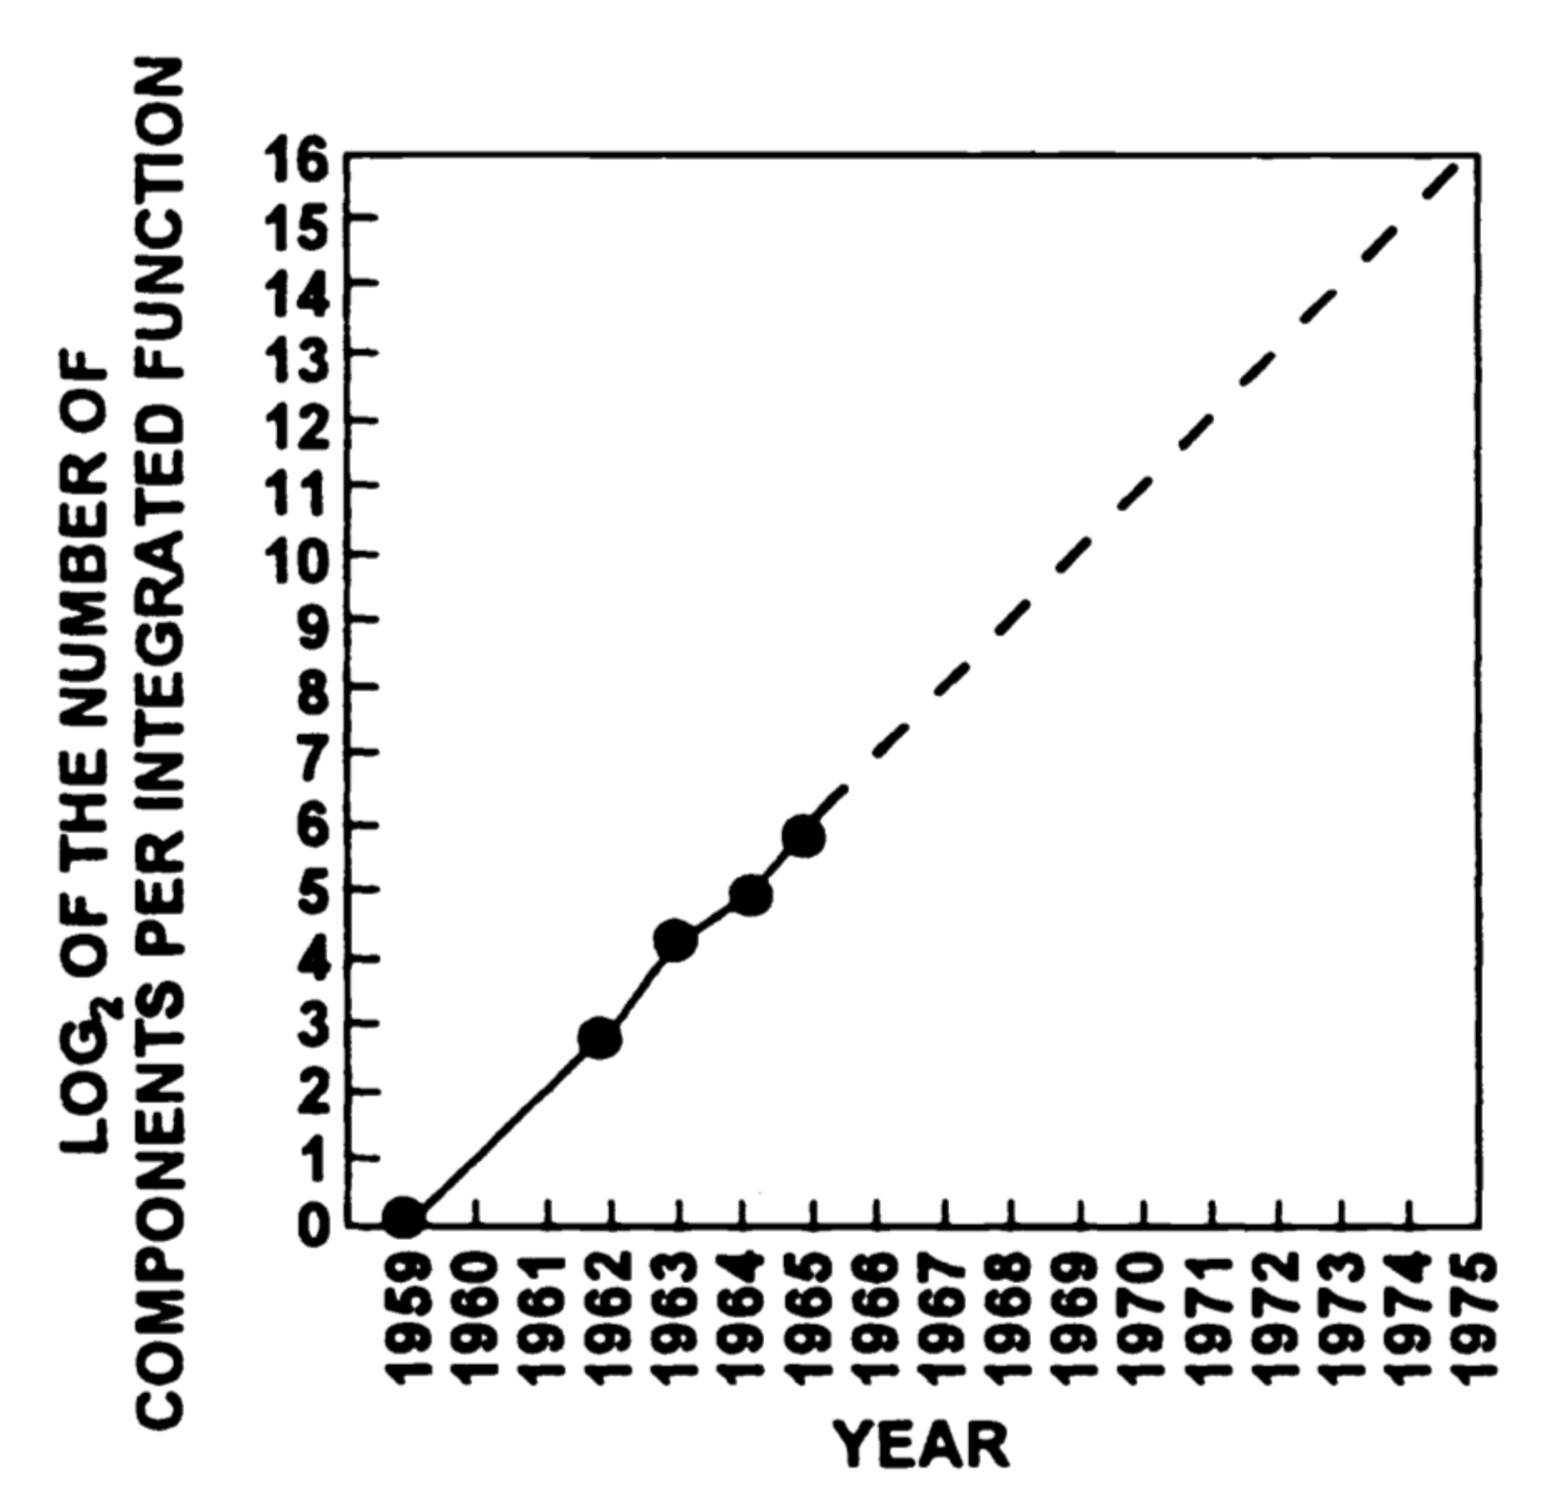
\includegraphics[width=0.7\textwidth]{images/original_moore.eps}
\caption{Original illustration of ``Moor's Law''. Figure taken from \cite{moore_cramming_1965}.}
\label{fig:moore_original}
\end{figure}

\begin{figure}
\centering
% l b r t
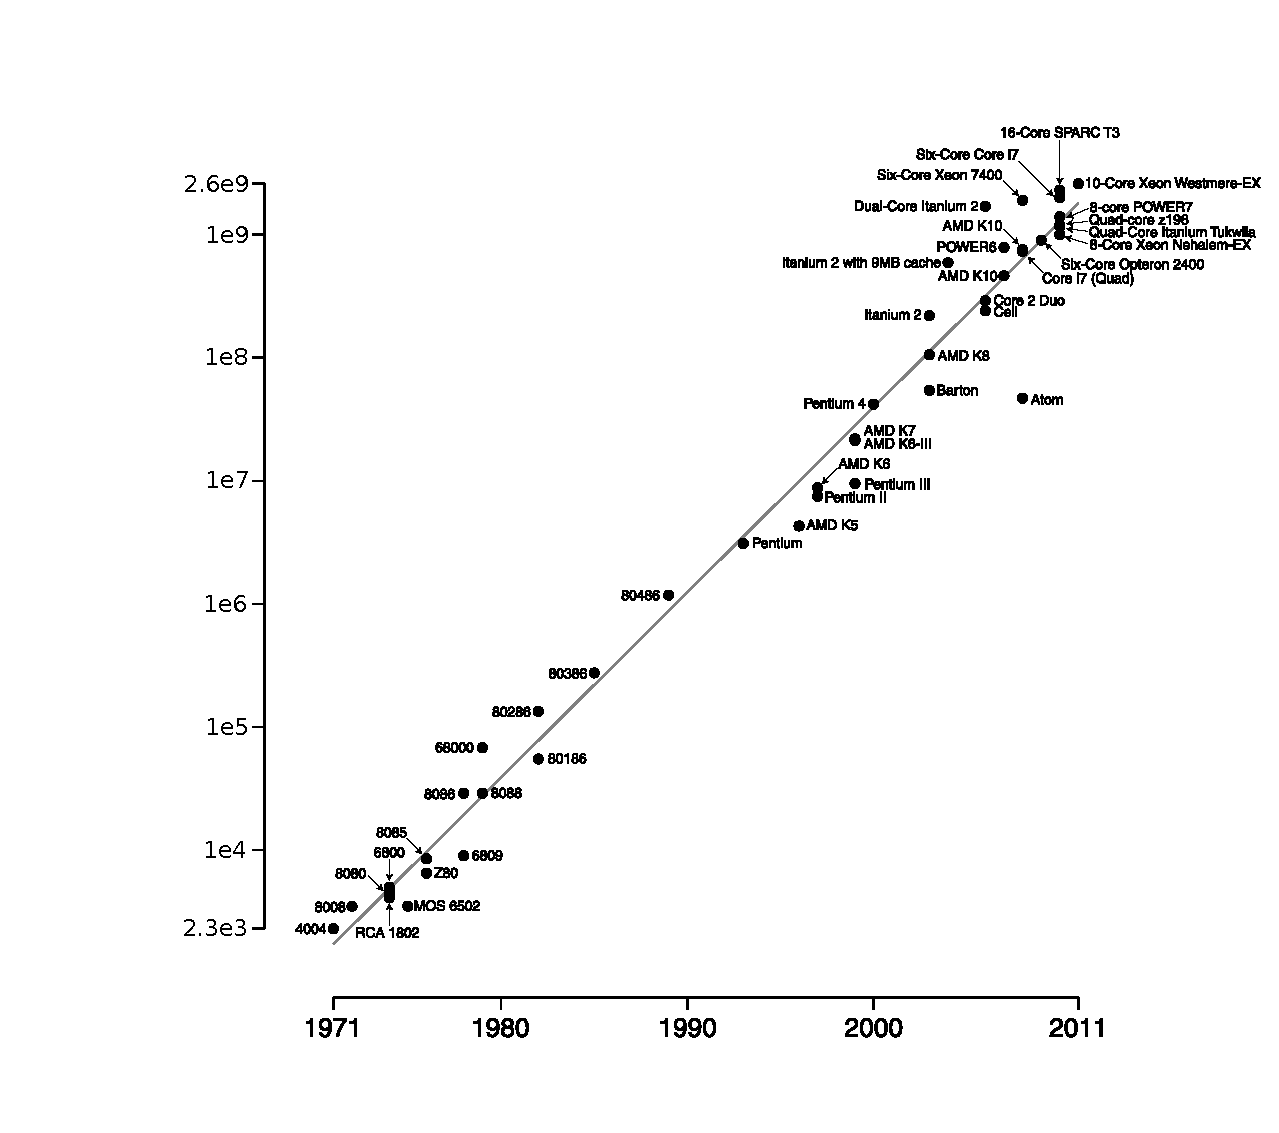
\includegraphics[trim = 20mm 10mm 0mm 0mm, clip,width=0.95\textwidth]{images/TransistorCount.eps}
\caption{Transistor counts of selected microprocessors introduced in the years 1971-2011. The diagonal line represents Moore's law. Figure taken from \cite{wgsimon_transistor_2011} (modified).}
\label{fig:moore_data}
\end{figure}

In the emerging field of computational biochemistry two fundamentally different approaches are used to derive the dynamic evolution of a system over time from a mathematical model: deterministic and stochastic simulation. The former, often considered the `classical' way, is based on a macroscopic description of the reactive species. The system is represented by a set of differential equations which can be solved numerically to gain insight into its dynamic behaviour. The latter, a more recently proposed and popularized approach, is based on the intrinsic randomness chemical species are subject to on a microscopic level. In the context of probability theory and statistics, the next reaction to fire as well as the according point in time can be modeled by means of correctly-distributed random variables. 

Over the course of centuries numerous fundamental theoretical results and efficient numerical methods for solving differential equations have been presented. Today, in consequence, systems of reasonable size can be solved accurately on affordable computing hardware in a relatively short amount of time. On the other hand, deterministic methods are considerably more expensive from a computational point of view. Furthermore, for system configurations where macroscopic concepts such as concentration are a valid approximation to the microscopic system dynamics, the averaged results of stochastic simulations often converge to the deterministic solution. One may therefore be tempted to question the relevance of the stochastic approach in practice. However, in cases where system dynamics is dominated by the particles of one or more species available only in small quantities, deterministic models cannot be used. In fact stochastic algorithms are needed to correctly simulate the temporal evolution of most biological systems. Stochastic effects arising from small molecular concentrations can only be considered by a non-deterministic approach. Examples of successful applications include genetics \cite{mcadams_stochastic_1997}, cellular signal transduction \cite{erban_signal_2005} and drug delivery \cite{ford_multi-scale_2011}. 

In practice a great variety of these processes can be modeled in terms of reaction and diffusion. Particles close to one another can collide and react according to prescribed reaction channels. Diffusion, on the other hand, macroscopically describes the spatial movement of molecules in the direction of the negative concentration gradient due to microscopic effects such as Brownian motion. The methods presented in the framework of this thesis are applicable for generic reaction-diffusion systems. To maintain a reasonable scope, however, a special focus is placed on the Gray-Scott model \cite{gray_autocatalytic_1984, pearson_complex_1993}. This primary example is of great interest due to its ability to exhibit pattern formation caused by an embedded activator-inhibitor process. Pattern formation as a form of self-organization ``can be considered the complement of the second law of thermodynamics\footnote{"The entropy of a closed system never decreases"} explaining the emergence of order from disorder instead of disorder from order'' \cite{mainzer_local_2013}. In practice this mechanism was observed in follicle spacing on mice skin \cite{sick_wnt_2006}. It can be used to describe pigmentation pattering in mammals \cite{murray_mathematical_2002}. Reaction-diffusion models have recently been used to simulate signalling pathways in eukaryotic cells \cite{takahashi_spatio-temporal_2010}. 

For his original prediction Moore considered a time span of ten years into the future (see figure \ref{fig:moore_original}). As of today (July 2014), Moor's Law is still considered to be valid \cite{techradar_moores_2014}. However, it is a common misunderstanding that computing power of microprocessors doubles at the same rate. Not the level of integration is the main driver of performance, but the processor's clock speed is. The latter has an enormous influence on the system's energy efficiency and since it is bound by the amount of heat a CPU cooler can dissipate, (starting in around 2005/06) a novel approach was introduced to the mainstream market: multi-core CPUs. This paradigm shift requires developers to explicitly write code that can make use of multiple parallel execution units. Another more recent trend in scientific computation is General-purpose Computing on Graphics Processing Units (GPGPU). Considering raw computational power (i.e.\ the number of floating point operations per second, FLOP/s) GPUs easily outperform CPUs. 

Due to the great computational complexity of stochastic simulation algorithms parallel platforms must be considered in order to simulate systems whose enormous complexity was previously considered prohibitive. In this thesis a simulator is presented that can make use of both, multi-core CPU and GPU, to accelerate stochastic reaction-diffusion simulations. The implementation depends on the OpenMP standard and Nvidia CUDA, respectively. Even though optimization techniques were used and the results of performance analysis is given, this work will not answer the question of which platform is suited better for stochastic simulations. The presented application is far from being perfect on both platforms. The goal of the project is merely to give an overview about available techniques and demonstrate results that can be achieved in a time-limited academic project. 

The structure of this thesis is as follows: In chapter 1, a compact overview about the topics and the scope of this thesis was given. In chapter 2, theoretical aspects of both approaches are derived and important results are cited. It is therefore the foundation for the two following chapters: In chapter 3, the implementation details and ideas incorporated into the developed programmes as well as the platforms they are targeted at are presented. In the subsequent chapter the tools are validated by comparison to analytic solutions of model examples. In addition, the more complex Gray-Scott model is simulated to assess performance on the different platforms and to demonstrate the pattern formation mechanism. The final chapter briefly summarizes the results of the thesis and gives an outlook on possibilities, trends and ideas to further improve the presented methods.